\scanpage{606}

\deleted{\unsure{Pour avoir}} \inserted{La relation} (99),
\deleted{il \unsure{suffit} d'\unsure{avoir}} s'écrit
\[
\tag{102}
\left\{\begin{aligned}
\deleted{\det}\sigma a&\equiv u\quad
(\mathrm{SL}(2,\widehat{\mathbb Z}))\quad\text{i.e.}\quad
\det\sigma a=\det u\quad\text{i.e. (98)}\\
\sigma a&\equiv u\quad(\deleted{4}2)
\end{aligned}\right.
\]
\deleted{\unsure{i.e.}} et cette dernière congruence s'écrit
\[
\tag{103}\begin{gathered}
c\equiv0\quad(\deleted{4}2)\qquad d\equiv1\quad(\deleted{4}2)
\\[3pt]
\left(-d\equiv\mu\quad(\deleted{\unsure{4}}2)\ \text{\unsure{en est une conséquence}}
\ \text{car }\mu\equiv1\equiv-1\quad(2)\right).
\end{gathered}\]

NB On ne \unsure{peut avoir les} \deleted{\illegible{3} $\mu\equiv-1\ (4)$, car}
congruences \uline{mod 4}
$(\sigma a\equiv u\ (4)$, car on aurait
$\mu\unsure{\equiv}-d\equiv-1\ (4)$, ce qui est contraire à l'hypothèse
(95) $\mu\equiv1\ (4)$.

\deleted{Ainsi (102) est \unsure{trop fort}. Néanmoins, il \uline{faut}
(pour avoir (99)) qu'on ait
\[
\tag{102 bis}
\sigma a\equiv u\quad(2)\qquad\text{i.e.}
\]
\[
\tag{103 bis}
c\equiv0\quad(2),\qquad d\equiv1\quad(2)
\]
(la relation $-d\equiv\mu\ (2)$ en est une conséquence, car
$\mu\equiv1\equiv-1\ (2)$). \unsure{Ce}}

Revenant à la relation (99), on trouve ceci :

\deleted{\uuline{Proposition}} \inserted{Lemme.} Soient
$c,d\in\widehat{\mathbb Z}^{\deleted{\unsure{*}}}$ satisfaisant
\[
\tag{104}
\mu\overset{\mathrm{dfn}}{=}-(c^2+cd+d^2)\in\widehat{\mathbb Z}^{*}
\]
\margin{\uline{NB} On aura néc.\textsuperscript{t} $\mu\equiv-1\ (3)$}
\[
\tag{105}
\mu\equiv1\quad(4)\qquad
(\text{i.e. }c^2+cd+d^2\equiv-1\quad(4)).
\]
\[
\tag{106}
c\equiv0\quad(2),\qquad d\equiv1\quad(2)
\]
Soit \deleted{\unsure{a c|a=}} \inserted{\unsure{d}}
\[
\tag{107}
a=\tau'(c\rho+d)=
\begin{pmatrix}-c&c+d\\d&c\end{pmatrix}
\in\mathrm{GL}(2,\widehat{\mathbb Z})
\]
(matrice de déterminant $\mu$). Alors on a une congruence
\[
\tag{108}
a\tau'(a)^{-1}\equiv\varepsilon\qquad
\mathrm{mod}\ \widehat{\Pi}_0\subset\mathrm{GL}(2,\widehat{\mathbb Z})
\]
\deleted{\unsure{et}} le signe $\varepsilon\in\{\pm1\}$ ne dépend pas des
choix faits pour $c,d$.

\scanpage{607}
\mspage{607}

C'est le moment de le calculer ! Reprenant
\[
a_0=c\rho+d\quad\in Z_\rho
\]
on aura
\[
a=\tau'a_0,\quad \tau'(a)=a_0\tau',\quad
a\tau'(a)^{-1}=\tau'a_0\tau'^{-1}a_0^{-1}=\tau'(a_0)a_0^{-1}
\]
où
\[
\left\{\begin{aligned}
\tau'(a_0)&=c\rho^{-1}+d={}^{t}a_0\\
a_0^{-1}&={}^{t}a_0/\det a_0=-\frac1\mu(c\rho^{-1}+d)
\end{aligned}\right.
\]
\margin{On \unsure{pose} \inserted{pour
$\unsure{u\in}\mathrm{M}_2(\widehat{\mathbb Z})$}
${}^{t}u=(\mathrm{Tr}\,u)-u$ et on a ${}^{t}\rho=\rho^{-1}$
(plus généralement ${}^{t}u=u^{-1}$ si $\det u=1$)}
donc
\[
a\tau'(a)^{-1}=\tau'(a_0)a_0^{-1}
=-\frac1\mu(c\rho^{-1}+d)^2
=\frac1{c^2+cd+d^2}(c\rho^{-1}+d)^2
\]
Or on a
\[
(c\rho^{-1}+d)^2
=c^2\underbrace{\rho^{-2}}_{-\rho}
+2cd\underbrace{\rho^{-1}}_{1-\rho}+d^2
=-(c^2+2cd)\rho+(2cd+d^2).
\]
Or \deleted{comme}
\[
\begin{aligned}
c\equiv0\quad(2)&\Longrightarrow c^2,2cd\equiv0\quad(4)
\qquad\text{\deleted{donc}}\\
d\equiv1\quad(2)&\Longrightarrow d^2\equiv1\quad(4)
\qquad\text{donc}
\end{aligned}
\]
\deleted{
\[
a\tau'(a)^{-1}\equiv\unsure{\pm}1\quad(4)
\qquad\text{\unsure{a fortiori a}}
\]
}
\[
(\unsure{*})\qquad (c\rho^{-1}+d)^2\equiv1\quad(4)
\]
\deleted{d'autre part.}

\deleted{donc le signe $\varepsilon$ est égal à \uline{$+1$}.}

Et comme par hypothèse
\[
c^2+cd+d^2\equiv-1\quad(4)
\]
on aura
\[
\tag{109}
a\tau'(a)^{-1}=\frac1{c^2+cd+d^2}(c\rho^{-1}+d)^{\unsure{2}}
\equiv-1\quad(4)
\]
Donc on a prouvé, en fait

\uline{Proposition} Soient $c,d\in\unsure{\mathbb Z|\widehat{\mathbb Z}}$
tels que $\xi\overset{\mathrm{dfn}}{=}c^2+\unsure{cd}+d^2
\in\widehat{\mathbb Z}^{*}$, soit
\[
a=\tau'(c\rho+d)=\begin{pmatrix}-c&c+d\\d&c\end{pmatrix}
\in\mathrm{GL}(2,\widehat{\mathbb Z}),
\]
\deleted{\unsure{démontrons|supposons}}
\[
\deleted{(\unsure{110})}\qquad
\deleted{a\tau'(a)^{-1}}\inserted{\sigma a}
\equiv\begin{pmatrix}\xi&0\\0&1\end{pmatrix}
\quad(2)\qquad\text{i.e.}
\]
\figure{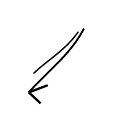
\begin{tikzpicture}[baseline]
\draw[line width=.65pt] (.8,.95) .. controls (.63,.62) and (.36,.43) .. (.1,.14);
\draw[line width=.8pt] (.1,.14)--(.34,.23) (.1,.14)--(.25,0);
\draw[line width=.5pt] (.73,.91) .. controls (.56,.67) and (.35,.56) .. (.16,.38);
\end{tikzpicture}}
\margin{\uline{NB} $\sigma=\begin{pmatrix}0&-1\\1&0\end{pmatrix}$}
\[
c\equiv0\quad(2),\qquad d\equiv1\quad(2).
\]

\scanpage{608}

Alors on a (pour $\tau'=\begin{pmatrix}-1&0\\0&1\end{pmatrix}$)
\[
a\tau'(a)^{-1}\equiv\varepsilon_2(\xi)\quad(4)
\]
(a fortiori on a la congruence mod $\widehat{\Pi}_0$).

\uline{Corollaire} L'extension $\mathcal E$ de $\mu\times\mu$ par $\mu$
(\unsure{84|89}), ou de $\mu$ par $\mathcal E''\simeq\mathbb Z/4\mathbb Z$, est non
commutative.
\margin{$\big|$}

Mais voici une façon de le voir sans calcul. Si l'extension était commutative,
\deleted{elle} \inserted{sa classe d'isomorphie} serait donnée par un
$\unsure{\mathrm{Ext}_{\mathbb Z}|\mathrm{Ext}^1_{\mathbb Z}}$
(ou un $\mathrm{Ext}^{\unsure{1|?}}_{\mathbb Z/4\mathbb Z}$).
Or le foncteur $\unsure{\mathrm{Ext}|\mathrm{Ext}^1}(-,\mu)$ est additif. Comme la restriction de
l'extension aux ss-groupes $\mathcal E'/\mu$ et $\mathcal E'''/\mu$ de
$\mu\times\mu$ est trivial, et que $\mu\times\mu$ est
la somme directe de ces sous-groupes (qui sont resp. $1\times\mu$ et le
sous-groupe diagonal), il s'ensuivrait que l'extension serait
trivial, or on a vu que ce n'est pas le cas.

\deleted{\unsure{En|Et}} \unsure{La} structure du groupe $\mathcal E$
s'explicite aisément, p.ex. en \unsure{tant} qu'extension de
$\mathcal E/\mathcal E''\simeq\mu$ par
$\mathcal E''\simeq\mathbb Z/4\mathbb Z$. \deleted{Soit}
Choisissons un élément quelconque de $\mathcal E-\mathcal E''$, il est
d'ordre 2 (les seuls élémts d'ordre 4 étant dans $\mathcal E''$) de sorte
que l'on a

\scanpage{609}
\mspage{608}

\[
\tag{110}
\mathcal E\simeq\{1,x\}\mathbin{.}\mathcal E''
\qquad\left(\tfrac12\ \text{direct}\right)
\]
Notons que si $x$ opérait trivialement sur $\mathcal E''$,
\deleted{i.e.} si $\mathcal E$ était isomorphe au produit, alors pour un
élément \inserted{$u$ de $\mathcal E''$} d'ordre 4,
$x.u$ serait d'ordre \unsure{4|8}, ce qui est absurde (troisième démonstration du fait
que \inserted{$\mathcal E/\mathcal E''\simeq$} $\mu$ opère non-trivialement
sur $\mathcal E''$). Or du seul fait que l'op. de $\{1,x\}$ sur
$\mathcal E''$ est non triv\unsure{.}, elle est connue, et
\inserted{la structure de} $\mathcal E$ est déterminée -- en fait on a
\[
\tag{\unsure{111|110}}
\mathcal E\simeq\mathbb D_4
\]
Il y a un choix privilégié de $x$, en prenant pour $x$ l'élém\unsure{t}
\[
\tag{112}
\left\{\begin{aligned}
\tau_{\mathcal E}&\overset{\mathrm{dfn}}{=}
\tau_{\unsure{S_0\Gamma}}\ \mathrm{mod}\ S_0^{\Pi}\Gamma^0,
\quad\text{où bien sûr}\\
\tau_{S_0\Gamma}&=(\tau,\tau',\tau),
\end{aligned}\right.
\]
de sorte que l'on a une représentation canonique
\[
\tag{113}
\mathcal E\simeq\{1,\tau_{\mathcal E}\}\mathbin{.}
\mathcal E''
\qquad\text{produit }\tfrac12\text{ direct}
\]
\margin{$\mathcal E''\simeq\mathbb Z/4\mathbb Z$\quad
$\tau_{\mathcal E}(u)=u^{-1}$ pour $u\in\mathcal E''$.}

L'hom $\mathcal E\to\mu\times\mu$ se récupère par ses restrictions aux
deux facteurs
\[
\tag{114}
\diagram{\begin{tikzcd}[column sep=large,row sep=large,column sep=9pt,row sep=14pt,execute at begin picture={\fontsize{10}{12}\selectfont}]
\mu\simeq\{1,\tau_{\mathcal E}\}\arrow[r]&\mu\times\mu&
\tau_{\mathcal E}\arrow[r,mapsto]&(-1,-1)\quad\text{(hom diagonal)}\\
\mathcal E''\arrow[r]&\unsure{\mu\times\{1\}}\arrow[r,hook]&\mu\times\mu&
\end{tikzcd}}
\]
l'unique hom non trivial $\mathcal E''\to\mu$ déduit de l'isom
\[
\diagram{\begin{tikzcd}
\mathcal E''_2\overset{\mathrm{dfn}}{=}
\unsure{\mathcal E''/2\mathcal E''|\mathcal E''/{}_{2}\mathcal E''}
\arrow[r,"\sim"]&\mu
\end{tikzcd}}
\]

\scanpage{610}

Le fait que $\mathcal E$ ne soit pas commutative s'exprime aussi par le fait
que l'hom can
\[
\tag{115}
\diagram{\begin{tikzcd}
\mathcal E_{\mathrm{ab}}\arrow[r,"\sim"]&\mu\times\mu
\end{tikzcd}}
\]
est un iso, i.e. que le sous-groupe noyau $\mu$ de
$\unsure{\mathcal E_{\mathrm{ab}}|\mathcal E}\to\mu\times\mu$ est aussi
le sous-groupe des commutateurs.

On a vu que l'extension $\mathcal E$ de $\mu\times\mu$ par $\mu$ n'est pas
scindée, mais qu'en est-il de son image inverse, l'extension
$S_0^{\Pi}\Gamma^!$ de $Z^!\simeq\mathcal M[0]$ par $\mu$ ? A priori,
on sait seulement qu'il n'y a pas de scindage de cette extension qui
prolonge le scindage canonique $A$ dont on dispose au dessus de
\[
Z^0=\mathrm{Ker}\left(\diagram{\begin{tikzcd}
Z^!\arrow[r,"(\varepsilon_3,\varepsilon_2)"]&\mu\times\mu
\end{tikzcd}}\right).
\]
Je présume que $\overline{\mathrm m}$ $S_0^{\Pi}\Gamma''$, extension de
$Z^{!\unsure{\prime\prime}}$ par $\mu$, est non triviale, et
$\overline{\mathrm m}$ l'extension qu'elle induit au sous-groupe
\[
\Gamma'_{\mathbb Q}=\Gamma_{\mathbb Q}\cap
\underbrace{\Gamma_{\mathbb Q}^{\prime\sim}}_{\substack{\wr\\\mathcal M(0)'}}
\subset\mathcal M^{\unsure{\xi|*}}(0)\subset\mathcal M^![0]=Z^!.
\]
Il serait intéressant d'identifier, \deleted{l'ext}
plus précisément, l'extension sur $\Gamma_{\mathbb Q}$, qu'elle induit, qui
correspond à un élément canonique
\[
\tag{115}
c\in H^{\unsure{2}}(\mathrm{Spec}\,\mathbb Q,\mu_2)\subset\mathrm{Br}(\mathbb Q)
\]

\scanpage{611}
\mspage{609}

Sauf erreur on aura
\[
\tag{115}
c=\underset{\text{(cup-produit)}}{\xi'\xi''},
\quad\text{où}\quad
\xi',\xi''\in
H^2(\mathbb Q,\unsure{\mu_2})
\]
sont les éléments qui décrivent respectivement les extensions
$\mathbb Q(\sqrt[3]{1})=\mathbb Q(\sqrt{-3})$, et
$\mathbb Q(\sqrt{3})$ --- contenues l'une et l'autre, ainsi que
$\mathbb Q(\sqrt{-1})=\mathbb Q(i)$, dans l'extension biquadratique
$\mathbb Q\bigl(\underset{\substack{\Vert\\\sqrt[2]{-1}}}{i},
\underset{\substack{\Vert\\\sqrt[3]{1}}}{j}\bigr)
=\mathbb Q(\sqrt[12]{1})$, le corps des racines
$12^{\text{ièmes}}$ de l'unité (dont le groupe de Galois est
$(\mathbb Z/12\mathbb Z)^*\simeq(\mathbb Z/3\mathbb Z)^*\times
(\mathbb Z/4\mathbb Z)^*\simeq\mu\times\mu$).

Il doit être trivial --- quand on \unsure{connaît} un peu les fondements ---
que $c$ ainsi explicité est $\ne0$, et n'est pas non plus
\unsure{scindé} en passant à $\mathbb Q(i)$, le troisième larron.

\figure{\begin{tikzpicture}\draw (0,0)--(2,0);\end{tikzpicture}}

Considérons maintenant le $\mu$-\unsure{groupement} central
\margin{\uline{NB} $Z\simeq\mathcal M[0]$, $\gamma\simeq\widetilde{\Gamma}_{\mathbb Q}$}
\[
\tag{116}
\diagram{\begin{tikzcd}[column sep=large]
\mu \arrow[r,hook,"i_{\rho,\mu}"] &
S_0\Gamma^!_{\rho,\sigma}
=Z^!_{\rho,\sigma}\times_\gamma N^*_\rho\times_\gamma N^*_\sigma\\
\varepsilon \arrow[r,mapsto] & (1,\varepsilon,1)
\end{tikzcd}}
\]
à valeurs dans
\[
\operatorname{Ker}(S_0\Gamma^!_{\rho,\sigma}\longrightarrow
Z^!_{\rho,\sigma})\simeq L_\rho\times L_\sigma,
\]
on a donc un hom. canonique de relèvement
\[
\tag{117}
\diagram{\begin{tikzcd}[column sep=large]
\mathcal M^![0]\simeq Z^!_{\rho,\sigma}
\simeq S_0^\Pi\Gamma^!_{\rho,\sigma}/\mu
\arrow[r] & S_0\Gamma^!_{\rho,\sigma}/i_{\rho,\mu}(\mu),
\end{tikzcd}}
\]

\scanpage{612}

qui s'explicite en termes \unsure{\deleted{des}|des} deux hom.
canoniques fondamentaux
\margin{Ceci mérite d'être explicité dans un théorème récapitulatif $\ldots$}
\[
\tag{118}
\diagram{\begin{tikzcd}[column sep=large,row sep=small]
Z^!_{\rho,\sigma} \arrow[r,"\uline{a}"]
\arrow[d,phantom,"\simeq"{description,sloped}] & N^*_\rho/\mu,
& Z^!_{\rho,\sigma} \arrow[r,"\uline{b}"] & N^*_\sigma\\
\mathcal M[0] \arrow[d,phantom,"\simeq"{description,sloped}] &&&\\
\widetilde{\Gamma}_{\mathbb Q}\mathbin{.}L_0^{\unsure{\Pi}} &&&
\end{tikzcd}}
\]
où, je rappelle
\[
\tag{119}
\left\{\begin{array}{l}
N^*_\rho\subset\mathcal M=\widetilde N_{1,1}\simeq
\widetilde\Gamma_{\mathbb Q}\mathbin{.}
\underbrace{\mathcal G^+}_{\mathrm{SL}(2,\mathbb Z)^\wedge}\\
\Vert\\
\{u\in\mathcal M\mid
u(\rho)=\deleted{\text{\unsure{fixe le gr.}}}\rho^{\varepsilon_3(u)}\}\\[1ex]
\deleted{\unsure{\{}}N^*_\sigma\subset\mathcal M\\
\Vert\\
\{u\in\mathcal M\mid u(\sigma)=\sigma^{\varepsilon_2(u)}
\ (=\varepsilon_2(u)\sigma)\}.
\end{array}\right.
\]

Les applications $\uline{a},\uline{b}$ sont données par les formules (cf 51)
\[
\tag{120}
\left\{\begin{array}{ll}
\uline{a}(u)=a=\varepsilon_3[\tau']\alpha^{-1}u,
& \uline{b}(u)=b=\beta^{-1}u\quad\text{i.e.}\\
\alpha=ua^{-1}\varepsilon_3[\tau'],&\beta=ub^{-1}
\end{array}\right.
\]
où $\alpha\in\widehat\Pi_{0\tau}$, $\beta\in\widehat\Pi_0$
sont caractérisés par
\[
\tag{121}
u(\rho)=\operatorname{int}(\alpha)(\rho),\quad
u(\sigma)=\varepsilon_2(\sigma)\operatorname{int}(\beta)(\sigma).
\]
Les quantités \deleted{\unsure{$a,$}}
$a=\uline{a}(u)\inserted{\in N^*_\rho/\mu}$,
$b=\uline{b}(u)\inserted{\in N^*_\sigma}$ sont caractérisées en termes de
$u\in Z^!$ (à un signe près seulement) par les congruences
\[
\tag{122}
u\equiv b\quad(\widehat\Pi_0),\qquad
u\equiv\varepsilon_3[\sigma]a\quad(\widehat\Pi),
\]
qui impliquent a fortiori (réduisant mod $\mathcal G^{+\wedge}$),
qu'on a commutativité \unsure{du|de},

\scanpage{613}
\mspage{\unsure{619|610}}

\deleted{(\unsure{123|122})}
\[
\tag{123}
\diagram{\begin{tikzcd}[column sep=large,row sep=small]
&N^*_\rho/\{\unsure{\pm}1\}\arrow[dr,"\delta_\rho"]&\\
Z^!_{\rho,\sigma}\arrow[ur]\arrow[dr]
\arrow[rr,dashed,"\delta_Z"]&&\gamma_{\rho,\sigma}\simeq\widetilde\Gamma_{\mathbb Q}\\
&N^*_\sigma\arrow[ur,"\delta_\sigma"']&
\end{tikzcd}}
\]

\deleted{Considérons maintenant les deux $\mu$-groupements}
\[
\deleted{(124)}\qquad
\diagram{\begin{tikzcd}[column sep=large,nodes in empty cells]
\deleted{\mu}\arrow[r] &
\deleted{S_0\unsure{\mathcal M|\Gamma}_{\rho,\sigma}}
\end{tikzcd}}
\]

Il serait temps de rectifier la confusion (p.\ \unsure{594'}) entre
$Z=Z_{\rho,\sigma}\not\subset
\mathcal M_{0,3}^{\unsure{\circ|\bullet}\sim}$,
et $Z^!=Z^!_{\rho,\sigma}=\deleted{\unsure{\mathcal M}}
Z\cap\mathcal M_{0,3}^{!\sim}$.
On a en fait
\[
\tag{124}
\diagram{\begin{tikzcd}[column sep=small,row sep=large]
Z_{\rho,\sigma}^{\deleted{\unsure{!}}}\simeq
\underset{\frac12\text{-direct}}{\mathcal M^{\unsure{\xi}}(0)\mathbin{.}L_0^{\mathcal G}}
\subset\mathcal M\arrow[dr,"\sim"]&\\
&\mathcal M_{0,3}^{\unsure{\xi}\sim}(0)\mathbin{.}
L_0^{\mathcal G_{0,3}}\subset\widetilde{\mathcal M}_{0,3}
\end{tikzcd}}
\]
\[
\tag{125}
\diagram{\begin{tikzcd}[column sep=small,row sep=large]
Z^!_{\rho,\sigma}\simeq Z^!_{\rho,\sigma}\cap\mathcal M^!
=\underset{\frac12\text{-direct}}{\mathcal M(0)\mathbin{.}L_0^\Pi}
\subset\mathcal M\arrow[dr,"\sim"]&\\
&\widetilde{\mathcal M}_{0,3}(0)\mathbin{.}L_0^{\Pi_{0,3}}
\deleted{\unsure{\subset\widetilde{\mathcal M}_{0,3}}}
\inserted{(\subset\widetilde{\mathcal M}_{0,3})}
\end{tikzcd}}
\]

Le lien entre les deux est donné par le diagramme
\[
\tag{126}
\diagram{\begin{tikzcd}[column sep=small,row sep=large]
1\arrow[r]&L_0^\Pi\arrow[r]\arrow[d,hook]&
Z^!_{\rho,\sigma}\arrow[r]\arrow[d,hook]&
\gamma_{\rho,\sigma}\arrow[r]\arrow[d,equal]&1\\
1\arrow[r]&L_0^{\mathcal G}\arrow[r]&
Z_{\rho,\sigma}\arrow[r]&
\gamma_{\rho,\sigma}\arrow[r]
\arrow[d,phantom,"\simeq"{description,sloped}]&1\\
&&&\mathcal M(0)\simeq\widetilde\Gamma_{\mathbb Q}&
\end{tikzcd}}
\]
où $L_0^\Pi\longrightarrow L_0^{\mathcal G}$ est
l'inclusion d'indice $2$ de
\[
\tag{127}
\diagram{\begin{tikzcd}[column sep=large,row sep=small]
L_0^\Pi=\ell_0^{\widehat{\mathbb Z}}
\arrow[r,hook]\arrow[d,phantom,"="{description,sloped}]&
\deleted{\unsure{\ell_0^{\widehat{\mathbb Z}}|\varepsilon_0^{\widehat{\mathbb Z}}}}
L_0^{\mathcal G}=\varepsilon_0^{\widehat{\mathbb Z}}\\
\varepsilon_0^{2\widehat{\mathbb Z}}&
\end{tikzcd}}
\]
Bien entendu, c'est bien sur $Z^!_{\rho,\sigma}$, non sur
$Z_{\rho,\sigma}$, qu'on a défini (117), (118) d'où (123).

\scanpage{614}

Je m'intéresse à la restriction des hom (123) au sous-groupe
$L_0^\Pi$ de $Z^!_{\rho,\sigma}$
la caractérisation (122) montre que l'hom induit
\[
\diagram{\begin{tikzcd}[column sep=large]
L_0^\Pi\arrow[r]&N^*_\rho/\{\pm1\}
\end{tikzcd}}
\]
\deleted{est}
est trivial (car $a$ en termes de $u$ ne dépend que de $u$ mod
$\widehat\Pi$), tandis que l'hom induit
\[
\diagram{\begin{tikzcd}[column sep=large]
L_0^\Pi\arrow[r]&N^*_\sigma
\end{tikzcd}}
\]
se factorise par $L_0^\Pi/L_0^{\Pi_0}\simeq\mathbb Z/2\mathbb Z$
(car $b$ en termes de $u$ ne dépend que de $u$ mod $\widehat\Pi_0$).
Sa valeur \inserted{$b$} sur \deleted{$\varepsilon_0$} $\ell_0$ est
\deleted{donnée}\inserted{\unsure{caractérisée|caractérisé}}
par les conditions
\[
\unsure{\{}\qquad b\in N^*_\sigma,\qquad b\equiv\ell_0\quad(\Pi_0)
\]
qui sont satisfaites évidemment par $b=-1$. Donc
Il y a lieu d'introduire aussi, qu'on le veuille ou non, le
$\mu$-groupement central canonique
\[
\tag{128}
\diagram{\begin{tikzcd}[column sep=large]
\mu\arrow[r,hook]&N^*_\sigma\\
-1\arrow[r,mapsto]&-1
\end{tikzcd}}
\]
et on a commutativité de
\[
\tag{129}
\diagram{\begin{tikzcd}[column sep=large,row sep=large]
L_0^\Pi\arrow[r,hook]\arrow[d]&Z^!_{\rho,\sigma}\arrow[d]\\
L_0^\Pi/L_0^{\Pi_0}\simeq\mu\arrow[r,hook]&N^*_\sigma.
\end{tikzcd}}
\]
Donc on trouve, à partir des deux hom. (123),

\scanpage{615}
\mspage{611}

de $Z^!_{\rho,\sigma}$, par passage au quotient deux hom canoniques
\[
\tag{130}
\left\{
\diagram{\begin{tikzcd}[column sep=large,row sep=small]
\gamma_{\rho,\sigma}\arrow[r]\arrow[d,equal]&N^*_\rho/\{\pm1\}\\
\widetilde\Gamma_{\mathbb Q}\arrow[d,equal]&\\
\gamma_{\rho,\sigma}\arrow[r]&N^*_\sigma/\{\pm1\},
\end{tikzcd}}
\right.
\]
qui sont en fait des sections des
\[
\diagram{\begin{tikzcd}[column sep=large,row sep=small]
N^*_\rho/\{\pm1\}\arrow[r]&\gamma_{\rho,\sigma}\arrow[d,equal]&\\
&\widetilde\Gamma_{\mathbb Q}\arrow[d,equal]&\mathcal M(0)\arrow[l,"\sim"']\\
N^*_\sigma/\{\pm1\}\arrow[r]&\gamma_{\rho,\sigma},&
\end{tikzcd}}
\]
de sorte qu'on trouve des décompositions,
\[
\tag{131}
\left\{\begin{array}{l}
N^*_\rho/\pm1\simeq\gamma_{\rho,\sigma}
\deleted{\unsure{\ltimes|\times}}\mathbin{.}
\underbrace{SZ_\rho/\{\pm1\}}_{=L_\rho/\{\pm1\}\simeq\mathbb Z/3\mathbb Z}\\[2ex]
N^*_\sigma/\pm1\simeq\gamma_{\rho,\sigma}\mathbin{.}
\underbrace{SZ_\sigma/\pm1}_{=L_\sigma/\pm\ \simeq\mathbb Z/2\mathbb Z}
\end{array}\right.
\]
(produits $\frac12$-directs). L'opération de $\gamma_{\rho,\sigma}$ sur
$L_\rho/\{\pm1\}\simeq\mathbb Z/3\mathbb Z$ est donnée par le
caractère quadratique $\varepsilon_3$, celle sur
$L_\sigma/\{\pm1\}\simeq\mathbb Z/2\mathbb Z$ est donnée par le caractère
quadratique $\varepsilon_2$.

La symétrie de présentation des deux hom (130) est un peu
\unsure{bidon} --- p.ex. l'hom
$\widetilde\Gamma_{\mathbb Q}=\gamma_{\rho,\sigma}\longrightarrow
N^*_\sigma/\{\pm1\}$ se remonte de façon évidente en
\[
\tag{132}
\diagram{\begin{tikzcd}[column sep=small,row sep=large]
\widetilde\Gamma_{\mathbb Q}=\gamma_{\rho,\sigma}\arrow[rr]&&N^*_\sigma,&\\
&\mathcal M(0)\arrow[ul,"\sim"]
\arrow[rr,phantom,"\subset"{description}]&&\mathcal M[0]=Z^!\arrow[ul]
\end{tikzcd}}
\]

\scanpage{616}

Une autre façon de le voir est de noter que
\[
 (132)\qquad \gamma_{\rho,\sigma}\simeq
 \mathcal M_0^{\unsure{!}}[0]/L_0^{\Pi_0}
\]
où
\[
 \mathcal M_0^{\deleted{\unsure{*}}!}[0]
 \overset{\mathrm{dfn}}{=}
 \mathcal M_{\unsure{\delta|0}}(0).L_0^{\Pi_0}
 \underset{\substack{\text{ss-groupe}\\\text{d'indice }2}}{\subset}
 \mathcal M^![0]=\mathcal M(0).L_0^{\unsure{\Pi|\tau}}
\]

Or sur $L_0^{\Pi_0}$, l'hom induit par
\diagram{\begin{tikzcd}
 \mathcal M^![0]=Z^!_{\rho,\sigma} \arrow[r] & N^*_{\sigma}
\end{tikzcd}}
est trivial. Ainsi on a $\overline{\mathrm m}$ un
\deleted{\unsure{isomorphisme}} scindage de
\[
 (133)\qquad
 \diagram{\begin{tikzcd}[column sep=large]
 1 \arrow[r] & L_{\sigma} \arrow[r] & N^*_{\sigma} \arrow[r]
 & \gamma_{\rho,\sigma} \arrow[r] \arrow[d, phantom, "\simeq" {rotate=90}] & 1\\
 &&& \widetilde{\Gamma}_{\mathbb Q}
 \end{tikzcd}}
\]
en un produit $\frac12$-direct
\[
 \deleted{\unsure{(134)}}\qquad
 N^*_{\sigma}\simeq\gamma_{\rho,\sigma}.L_{\sigma}
\]
qu'il vaut mieux écrire en concrétisant le sous-groupe section en
\unsure{tant} que ss-groupe de $G_{\rho,\sigma}\simeq\mathcal M$, soit donc
\[
\begin{aligned}
 (134)\qquad
 \unsure{N}_{0\sigma}^{!*}
 &\overset{\mathrm{dfn}}{=}
 \operatorname{Im}(\mathcal M_0[0]\longrightarrow N^*_{\rho})\\
 &=\operatorname{Im}(\mathcal M[0]\hookrightarrow N^*_{\rho})\\
 &=\{\beta^{-1}u\mid u\in\mathcal M(0),\ \beta\in\widehat\Pi_0
       \text{ tels que }u(\sigma)=\varepsilon_{\unsure{2}}(u)
       \operatorname{int}(\beta)(\sigma)\}\\
 &=\{v\in N^*_{\sigma}\mid \exists\,\beta\in\widehat\Pi_0\text{ tel que }
       \beta v\in\mathcal M[0]=\operatorname{Norm}_{\mathcal M}(\unsure{l_0})
       \cap\mathcal M^!\}
\end{aligned}
\]
\margin{\uline{NB} On définit $\mathcal M^!$ comme l'image inverse de
$\mathcal M_{0,3}^{!\sim}$, i.e. le noyau de la représentation canonique
\diagram{\begin{tikzcd}
 \mathcal M \arrow[r] &
 \underbrace{\mathcal G^{+\wedge}/\Pi^{\wedge}}_{\mathcal G_3}
 \arrow[r,"\sim"] &
 \operatorname{Aut}(\mathcal G^{+\wedge}/\Pi^{\wedge})
\end{tikzcd}}}

Posant
\[
 (135)\qquad
 \mathcal M_0^!\overset{\mathrm{dfn}}{=}\mathcal M(0).\Pi_0
 \underset{\substack{\text{indice}\\2}}{\subset}
 \mathcal M^!\overset{\mathrm{dfn}}{=}\mathcal M(0).\Pi,
\]

\scanpage{617}
\mspage{612}

de sorte qu'on a
\[
 (136)\qquad \mathcal M^!\simeq\mathcal M_0^!\times\mu,
\]
\margin{\uline{NB} On a
\diagram{\begin{tikzcd}
 \mathcal M_0^!\arrow[r,"\sim"] & \mathcal M_{0,3}^{!\sim}
\end{tikzcd}}}
on a donc
\[
 (137)\qquad
 \left\{\begin{aligned}
 N_{\sigma0}^{\deleted{\unsure{d}}*!}&=N^*_{\sigma}\cap\mathcal M_0^!\\
 N_{\sigma}^{*!}&\overset{\mathrm{dfn}}{=}N^*_{\sigma}\cap\mathcal M^!
                    =N_{\sigma0}^{*!}\times\mu,
 \end{aligned}\right.
\]
et on trouve que
\[
 (138)\qquad
 \diagram{\begin{tikzcd}
 N_{\sigma0}^{\unsure{*!|d!}}\arrow[r,"\sim"] &
 \gamma_{\rho,\sigma}=\widetilde\Gamma_{\mathbb Q}
 \end{tikzcd}}
\]
\deleted{\unsure{d'où}} Posons pour abréger
\[
 \deleted{(139)\qquad N_{\sigma}^{\unsure{d}}\simeq N_{\sigma0}^{*!}}
\]
\[
 (139)\qquad \mathcal M(1/2)=N_{\sigma0}^{*!}\qquad\text{cf }(137)
\]
on aura donc que $\mathcal M(1/2)$ est \unsure{un|une}
\inserted{\unsure{groupe-}}section
\deleted{(140)} pour $N_{\sigma}^{\unsure{*|\wedge}}$ extension de
$\gamma_{\rho,\sigma}$ par $L_{\unsure{\sigma|\rho}}$, et a fortiori pour
$\mathcal M$ ext. de $\gamma_{\rho,\sigma}$ par $\mathcal G^{+\wedge}$,
et \unsure{un|on} $\unsure{\overline{\mathrm m}|\simeq}$ \unsure{de plus|simples} pour
$\mathcal M_0^!,\mathcal M^!$
\[
 (140)\qquad
 \left\{\begin{aligned}
 \mathcal M_0^!&\simeq\mathcal M(1/2).\widehat\Pi_0\\
 \mathcal M^!&\simeq\mathcal M(1/2).\widehat\Pi\\
 \mathcal M&\simeq\mathcal M(1/2).\mathcal G^{+\wedge}\\
 N^*_{\sigma}&\simeq\mathcal M(1/2).L_{\sigma}
 \end{aligned}\right.
\]
\margin{$\longleftarrow$ attention, $\mathcal M^!$ est inv. dans $\mathcal M$
et $\mathcal M_0^!$ est inv. dans $\mathcal M^!$, mais
\uline{non dans} $\mathcal M$\quad cf plus bas}

[Si on veut \unsure{paraphraser} en introduisant
\[
 (141)\qquad
 N_{\rho0}^{*!}\overset{\mathrm{dfn}}{=}N^*_{\rho}\cap\mathcal M_0^!
 =\{v\in N^*_{\rho}\mid\exists\,\alpha\in\widehat\Pi_0\text{ tel que }
       \underbrace{\alpha v}_{u}\in\mathcal M(0)\}
\]
c'est donc l'un des $v$ qu'on peut associer au
$u\in\mathcal M(0)\subset\mathcal M^![0]=Z^!_{\rho,\sigma}$,
à l'aide des $\alpha\in\Pi_0$ tel que
$\alpha^{-1}u\in N_{\rho}^{\unsure{*|\wedge}}$ i.e.
\[
 u(\rho)=\operatorname{int}(\alpha)(\rho^{\varepsilon_3})
 \qquad\text{où}\quad\varepsilon_3=\varepsilon_3(u)=\varepsilon_3(v).
\]
Mais comme $u(\rho)$ doit avoir $\overline{\mathrm m}$ image dans
$\mathcal G_3=\mathcal G^{+\wedge}/\Pi$
que $\rho$, il faut qu'on ait $\varepsilon_3=1$, et alors
$\alpha$ est l'élément $\uline{\alpha}(u)$ associé à $u$ et
$v=\alpha^{-1}u$ est l'image can. de $u$ dans $N^{!*}_{\rho}$. Ainsi on

\scanpage{618}

trouve

\uline{Proposition} L'hom
$N_{\rho0}^{*!}\longrightarrow\gamma_{\rho,\sigma}=\widetilde\Gamma_{\mathbb Q}$
est injectif, et a pour image
$\gamma'_{\rho,\sigma}=\{\gamma\in\gamma_{\rho,\sigma}\mid\varepsilon_3(\gamma)=1\}$.

\uline{Corollaire}
$N_{\rho,0}^{*!}\subset Z_{\rho}^{\unsure{\xi|*}!}$ i.e.
$N_{\rho0}^{*!}=\deleted{\unsure{N}}Z_{\unsure{0\rho|\rho0}}^{\unsure{\xi|*}!}
 \overset{\mathrm{dfn}}{=}Z_{\rho}^{\unsure{\xi|*}}\cap\mathcal M_0^!$.

Il est naturel de poser
\[
 (142)\qquad N_{\rho0}^{*!}=Z_{\rho0}^!=\mathcal M(-\bar j)\,\unsure{..|.}
\]
Comme $N_{\rho}^{*!}\supset Z_{\rho}^!\supset\mu$, on voit que l'on a
\[
 (142)\qquad
 \left\{\begin{array}{rcll}
 N_{\rho\deleted{\unsure{0}}}^{*!}&=&N_{\rho0}^{*!}\times\mu
     &\bigl(\text{donc }N_{\rho}^{*!}=Z_{\rho}^!\bigr)\\
 \Vert&&&\\[-1ex]
 Z_{\rho}^!&=&Z_{\rho\unsure{0}}^!\times\mu&
 \end{array}\right.
\]
\[
 \deleted{\unsure{N_{\rho}}\simeq}
\]

Le sous-groupe $Z^!_{0,\rho}=\mathcal M(-\bar j)$ est une section de
$\mathcal M'$ sur $\gamma'_{\rho,\sigma}\simeq\Gamma_{\mathbb Q}^{\prime\sim}$,
et \deleted{\unsure{est}} \inserted{\unsure{$\mathcal M'$}}
\unsure{contenue|contenu} dans
\deleted{$Z^!_{0\rho}$ a fortiori dans}
$\mathcal M_0^{\prime!},\mathcal M^{\prime!},
 \deleted{\unsure{Z_{0\rho}}},Z_{\rho}^!,Z_{\rho}$,
on aura des décompositions en produit $\frac12$ direct
\[
 (143)\qquad
 \left\{\begin{aligned}
 \mathcal M_0^{\prime!}&\simeq\mathcal M(-\bar j).\Pi_0\\
 \mathcal M^{\prime!}&\simeq\mathcal M(-\bar j).\Pi\\
 \mathcal M^{\prime\unsure{\xi|*}}&\simeq\mathcal M(-\bar j).\mathcal G\\
 Z_{\rho}^!&\simeq\deleted{Z}\mathcal M^{\unsure{\xi|*}}(-\bar j)\times\mu\\
 Z_{\rho}^{\unsure{\xi|*}}&\simeq\mathcal M^{\unsure{\xi|*}}(-\bar j)\times L_{\rho}
 \qquad ....
 \end{aligned}\right.
\]
]

\deleted{Notons maintenant que}
\[
 \deleted{\mu_{\tau'}\overset{\mathrm{dfn}}{=}\{1,\tau'\}\subset\mathcal G^{\wedge}}
\]
\deleted{normalise $L_{\rho}$, donc $Z_{\rho}$, donc
$Z^!_{0,\rho}=Z_{\rho}\cap\mathcal M_0^!$}

\scanpage{619}
\mspage{613}

Revenons au diagramme (130), je dis que l'hom
\diagram{\begin{tikzcd}
 \gamma_{\rho,\sigma}\arrow[r]\arrow[d,phantom,"\Vert"] & N^*_{\rho}/\{\pm1\}\\
 \Gamma_{\mathbb Q}^{\sim}
\end{tikzcd}}
\uline{ne se relève pas} en un hom de $\gamma_{\rho,\sigma}$ dans
$\underset{\inserted{\widetilde\gamma_{\rho,\sigma}}}{N^*_{\rho}}$
--- en d'autres termes, que l'extension de $\gamma_{\rho,\sigma}$ par
$\{\pm1\}=\mu$ qu'elle définit n'est pas triviale. Pour identifier cette
extension, considérons le diagramme
\margin{\uline{NB}}
\[
(144)\qquad
\diagram{\begin{tikzcd}[column sep=large,row sep=huge,column sep=9pt,row sep=14pt,execute at begin picture={\fontsize{10}{12}\selectfont}]
 \mathcal M^![0]=Z^!_{\rho,\sigma}\arrow[rr,"\text{can}"]
 &&\gamma_{\rho,\sigma}=Z^!_{\rho,\sigma}/L_0^{\Pi}
       \arrow[r,"\text{hom }(130)"]
 &[60pt]N^*_{\rho}/\{\pm1\}\\
 S_0\Gamma^!_{\rho,\sigma}
       \arrow[u,"{\text{can}\quad(u,a,b)\mapsto u}"']
 &\inserted{\unsure{S_0}\Gamma_{\rho,\sigma}\quad\text{(sans !)}}
       \arrow[ur,very thick,"{\substack{\text{can}\\\unsure{\text{(passage au quotient)}}}}"']
 &&\\
 S_0^{\Pi}\Gamma^!_{\rho,\sigma}\arrow[u,hook,"\text{incl.}"']
       \arrow[ur,hook,dashed,"\text{incl.}"']\arrow[rrr]
 &&&N^*_{\rho}\arrow[uu]
\end{tikzcd}}
\]
qui montre que l'on a un diagramme de carrés cartésiens
\[
(145)\quad\deleted{\unsure{(146)|(144)}}\qquad
\diagram{\begin{tikzcd}[column sep=large,row sep=huge]
 \mathcal M(0)\arrow[r,hook]\arrow[dr,phantom,"\mathrm I" description]
 &\mathcal M^![0]=Z^!_{\rho,\sigma}\arrow[r,"\text{épi}"]
       \arrow[dr,phantom,"\mathrm {II}" description]
 &\gamma_{\rho,\sigma}\arrow[r,hook]
       \arrow[dr,phantom,"\mathrm {III}" description]
 &N^*_{\rho}/\{\pm1\}\\
 \mathcal M(0)^{\sim}\arrow[u]\arrow[r,hook]
 &S_0^{\Pi}\Gamma^!_{\rho,\sigma}\arrow[u,"2"]\arrow[r]
 &\widetilde\gamma_{\rho,\sigma}\arrow[u,"2"]\arrow[r,hook]
 &N_{\rho}^{\unsure{*|d}}\arrow[u,"2"]
\end{tikzcd}}
\]
où $\mathcal M(0)^{\sim}$ est \unsure{définie|défini} comme l'extension de
$\mathcal M(0)$ par $\mu$ induite par l'ext.
$S_0^{\Pi}\Gamma^!_{\rho,\sigma}$ de $\mathcal M^![0]$,
qui s'identifie donc \unsure{aussi} à l'image \unsure{réc.|réci.} de

\scanpage{620}

l'ext. $\widetilde\gamma_{\rho,\sigma}$ de $\gamma_{\rho,\sigma}$ par $\mu$,
par l'isom. composé
\diagram{\begin{tikzcd}
 \mathcal M(0)\arrow[r,"\sim"] & \gamma_{\rho,\sigma}.
\end{tikzcd}}
Donc l'ext. $\widetilde\gamma_{\rho,\sigma}$ de $\gamma_{\rho,\sigma}$ par
$\mu$ s'identifie \unsure{nt.|nat.} à l'ext. $\mathcal M(0)^{\sim}$ de
$\mathcal M(0)$ par $\mu$ dont on s'est convaincu plus ou moins qu'elle
n'était pas triviale.

Voici une autre façon d'obtenir l'hom canonique
\diagram{\begin{tikzcd}
 \gamma_{\rho,\sigma}\arrow[r] & N^*_{\rho}/\pm1,
\end{tikzcd}}
et l'extension $\widetilde\gamma_{\rho,\sigma}$ de $\gamma_{\rho,\sigma}$.
Considérons
\[
 (146)\qquad N_{\rho}^{*!}=N^*_{\rho}\cap\mathcal M^!
\]
On a alors
\[
 (147)\qquad
 N_{\rho}^{*!}\cap\mathcal G^+
 =\operatorname{Ker}\bigl(N_{\rho}^{*!}\longrightarrow
     \underbrace{\gamma_{\rho,\sigma}}_{\Gamma_{\mathbb Q}^{\unsure{\sim}}}\bigr)
 =L_{\rho}\cap\Pi=\mu
\]
d'autre part le hom
\[
 (148)\qquad
 \diagram{\begin{tikzcd}
 N_{\rho}^{*!}\arrow[r] & \gamma_{\rho,\sigma}
 \end{tikzcd}}
 \quad\text{est \uline{épi}}
\]
Car \deleted{pour $\forall$} il suffit de voir que \inserted{pour}
$\forall\,u\in\mathcal M(0)$, il existe un élément de $N_{\rho}^{*!}$
qui lui est congru, \inserted{mod $\mathcal G$} Or on a
\[
 u(\rho)=\operatorname{int}(\alpha)(\rho)
 \deleted{=\unsure{\operatorname{int}(\alpha_0\varepsilon_3[\tau])(\rho)}}
\]
\inserted{avec $\alpha\in\deleted{\unsure{\widehat\Pi_{\tau}}}
 \widehat\Pi_{\tau}=\{1,\tau\}.\widehat\Pi$,}
si $\varepsilon_3(u)=1$ i.e. $\alpha\in\widehat\Pi$,
$\alpha^{-1}u\in\deleted{\unsure{Z}}Z_{\rho}\subset N^*_{\rho}$
fait l'affaire. Si \deleted{$\unsure{\varepsilon_3(u)=-1}$}
\inserted{$\varepsilon_3\unsure{=|\ne}-1$}, on a
\deleted{on a}
\[
 \deleted{\alpha=\alpha_0}\quad\alpha=\alpha_0\tau,\qquad\alpha_0\in\widehat\Pi.
\]
et on a
\[
 u(\rho)=\alpha(\rho)=
 \alpha_0\bigl(\underbrace{\tau(\rho)}_{\sigma(\rho^{-1})}\bigr)
 =\alpha_0(\sigma(\rho^{-1}))\quad\deleted{donc}
\]
donc
\[
 (\sigma^{-1}\alpha_0^{-1}u)(\rho)=\rho^{-1}
 \quad\text{donc}\quad\sigma^{-1}\alpha_0^{-1}u\in N^*_{\rho}.
\]
\unsure{OK.}

\scanpage{621}
\mspage{614}

Donc on a une suite \unsure{exacte}

\begin{samepage}
\( (149) \)\quad
\diagram{\begin{tikzcd}[column sep=small,row sep=small]
1 \arrow[r] & \mu \arrow[r] & Z_\rho^{*!} \arrow[r] & \gamma_{\rho,\sigma} \arrow[r] \arrow[d,phantom,"\rotatebox{90}{$\simeq$}"] & 1 \\
& & (\simeq\widetilde{\gamma}_{\rho,\sigma}) & \widetilde{\Gamma}_{\mathbb Q} &
\end{tikzcd}}
\end{samepage}

qui fait de $Z_\rho^{*!}$ une $\mu$-ext. de $\gamma_{\rho,\sigma}$,
d'où un hom can.

\diagram{\begin{tikzcd}
\gamma_{\rho,\sigma}\simeq Z_\rho^{*!}/\mu \arrow[r] & N_\rho^*/\mu
\end{tikzcd}}

qui, bien entendu, n'est autre que le premier hom (130).

$9^\circ)$ \uline{Récapitulation sur le cas universel}.

Finalement, j'ai l'impression que j'ai fait encore des longs détours et
\unsure{contorsions}, pour finalement me perdre dans les sables, et perdre un
peu le fil. Je vais donc récapituler ce qui me semble essentiel.

\textcircled{a}
\[
\begin{gathered}(1)\qquad Z_{\rho,\sigma}\simeq\mathcal M(0).L_0^{\mathcal G}
\inserted{=\mathcal M[0]}\ \deleted{\illegible{1}}\\[3pt]\inserted{
\text{(opérant sur }\widehat{\mathcal G}^{+}\text{ par op. induite par }\unsure{\text{l'adjoint}}\text{)}}
\end{gathered}\]

on distingue dedans un sous-\unsure{groupe} d'indice $2$
\[
(2)\qquad Z_{\rho,\sigma}^{!}\simeq\mathcal M(0).L_0^{\Pi}.
\]

\scanpage{622}

On a
\[
(3)\qquad \unsure{G}_{\rho,\sigma}\simeq\mathcal M
\]

et, \deleted{les hom} plus précisément, le diagramme

\begin{samepage}
\( (4) \)\quad
\diagram{\begin{tikzcd}[column sep=small,row sep=large]
1 \arrow[r] & L_0 \arrow[r] \arrow[d,hook] & Z_{\rho,\sigma} \arrow[r] \arrow[d,hook] & \gamma_{\rho,\sigma} \arrow[r] \arrow[d,equal] & 1 \\
1 \arrow[r] & \mathcal G_{\rho,\sigma}^{+\wedge} \arrow[r] & G_{\rho,\sigma} \arrow[r] & \gamma_{\rho,\sigma} \arrow[r] & 1
\end{tikzcd}}
\end{samepage}

s'identifie au diagramme

\begin{samepage}
\( (4\text{ bis}) \)\quad
\diagram{\begin{tikzcd}[column sep=small,row sep=large]
1 \arrow[r] & L_0^{\mathcal G} \arrow[r] \arrow[d,hook] & \overbrace{\mathcal M[0]}^{\inserted{\mathcal M(0).L_0^{\mathcal G}}} \arrow[r] \arrow[d,hook] & \widetilde{\Gamma}_{\mathbb Q} \arrow[r] \arrow[d,phantom,"\rotatebox{90}{$\simeq$}"] & 1 \\
1 \arrow[r] & \widehat{\mathcal G}^{+} \arrow[r] & \mathcal M \arrow[r] & \widetilde{\Gamma}_{\mathbb Q} \arrow[r] & 1.
\end{tikzcd}}
\end{samepage}

D'ailleurs, les hom

\begin{samepage}
\( (5) \)\quad
\diagram{\begin{tikzcd}[column sep=large,row sep=small]
& \mu \\
\gamma_{\rho,\sigma} \arrow[ru,"{\varepsilon_\gamma'=\varepsilon_\gamma^\rho}"] \arrow[r] \arrow[rd,"{\varepsilon_\gamma''=\varepsilon_\gamma^{\unsure{\rho|\sigma}}}"'] & \widehat{\mathbb Z}^{*} \\
& \mu
\end{tikzcd}}
\end{samepage}

s'identifient :

\begin{samepage}
\( (5\text{ bis}) \)\quad
\diagram{\begin{tikzcd}[column sep=large,row sep=small]
& & \mu \\
\widetilde{\Gamma}_{\mathbb Q} \arrow[r,Rightarrow,"\chi"] \arrow[urr,bend left=15,"\varepsilon_3"] \arrow[drr,bend right=15,"\varepsilon_2"'] & \widehat{\mathbb Z}^{*} \arrow[ur] \arrow[dr] & \\
& & \mu.
\end{tikzcd}}
\end{samepage}

\Needspace{8\baselineskip}
\begin{samepage}
\textcircled{b}\quad On a

\margin{$/$}
\[
(6)\qquad N_\sigma^*=
\left\{u\in\unsure{\mathcal M}\ \middle|\ u(\sigma)=\deleted{\unsure{\varepsilon_2(u)}}\sigma^{\varepsilon_2(u)}
\begin{aligned}
&\bigl(=\varepsilon_2(u).\sigma\bigr)\\
&\inserted{=\varepsilon_2[\tau](\sigma)}\\
&\inserted{=\varepsilon_2[\tau'](\sigma)}
\end{aligned}
\right\}
\]
\end{samepage}

\deleted{\unsure{Posons}} et
\[
(7)\qquad
\left\{\begin{aligned}
N_\sigma^*\cap\widehat{\mathcal G}
  &=\mathbb D_\sigma=\{1,\tau\}.L_\sigma=\{1,\tau'\}.L_\sigma\\
N_\sigma^*\cap\mathcal G^{+\wedge}
  &= L_\sigma\qquad(\simeq\mathbb Z/4\mathbb Z)\\
N_\sigma^*\cap\Pi&=\mu\\
N_\sigma^*\cap\Pi_0&=\{1\}
\end{aligned}\right.
\qquad .
\]

\scanpage{623}
\mspage{615}

Posons
\[
(8)\qquad
\left\{\begin{aligned}
\mathcal M_0^!&=\mathcal M(0).\Pi_0
\subset\mathcal M^!=\mathcal M(0).\Pi
=\operatorname{Ker}(\mathcal M\to\mathcal G_3)\\
\text{de sorte que}\qquad
\mathcal M^!&\simeq\mathcal M_0^!\times\mu
\end{aligned}\right.
\]

et
\[
(9)\qquad
\left\{\begin{aligned}
\mathcal M(1/2)
&\overset{\mathrm{dfn}}=
\deleted{\unsure{A}}N_{\sigma\deleted{\unsure{\rho}}0}^{*!}
\overset{\mathrm{dfn}}=
\deleted{\unsure{Z_\sigma\mathcal M_0}}N_\sigma^*\cap\mathcal M_0^!\\
N_\sigma^{*!}&=N_\sigma^*\cap\mathcal M^!
=\deleted{\unsure{\mathcal M(1/2)|\mathcal M(0)}\times\mu},
\end{aligned}\right.
\]

alors l'hom \deleted{\unsure{de}} $\mathcal M\to\gamma_{\rho,\sigma}$
induit un \uline{iso}

\begin{samepage}
\( (10) \)\quad
\diagram{\begin{tikzcd}
\mathcal M(1/2)=N_{\sigma0}^{*!} \arrow[r,"\sim"] & \gamma_{\rho,\sigma}
\end{tikzcd}}
\end{samepage}

donc on a des scindages en produits $1/2$ \unsure{directs}
\[
(11)\qquad
\left\{\begin{aligned}
.\ \mathcal M^{\deleted{\unsure{!}}}
  &\simeq\mathcal M(1/2).\mathcal G^{+\wedge}\\
\mathcal M^!&\simeq\mathcal M(1/2).\Pi\\
\mathcal M_0^!&\simeq\mathcal M(1/2).\Pi_0\\
N_\sigma^{*!}&\simeq\mathcal M(1/2)\times\mu\\
N_\sigma^*&\simeq\mathcal M(1/2).L_\sigma
\end{aligned}\right.\quad,\quad\text{et}
\]

\begin{samepage}
\( (12) \)\quad
\diagram{\begin{tikzcd}
\gamma_{\rho,\sigma} \arrow[r,"\sim"] & \mathcal M(1/2)=N_{\sigma0}^{*!} \arrow[r,hook] & N_\sigma^*.
\end{tikzcd}}
\end{samepage}

\figure{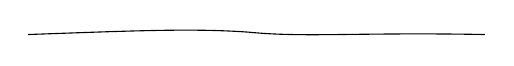
\begin{tikzpicture}
\draw (0,0) .. controls (1.4,.05) and (2.1,.08) .. (2.8,.03)
.. controls (3.5,-.04) and (4.2,.03) .. (5.8,0);
\end{tikzpicture}}

\textcircled{c}\quad On a
\[
(13)\qquad
N_\rho^*=\left\{u\in\mathcal M\mid u(\rho)=\rho^{\varepsilon_3(u)}\right\}
\quad\inserted{\bigl(=\varepsilon_3[\tau'](\rho)\bigr)}
\]

et
\[
(14)\qquad
\left\{\begin{aligned}
N_\rho^*\cap\widehat{\mathcal G}
  &=\mathbb D_\rho=\{1,\tau'\}.L_\rho\\
N_\rho^*\cap\mathcal G
  &=L_\rho\qquad(\simeq\mathbb Z/6\mathbb Z)\\
N_\rho^*\cap\Pi&=\mu\\
N_\rho^*\cap\Pi_0&=\{1\}
\end{aligned}\right.\qquad .
\]

\scanpage{624}

Soit
\[
(15)\qquad
N_{\rho0}^{*!}\overset{\mathrm{dfn}}=N_\rho^*\cap\mathcal M_0^!,
\qquad N_\rho^{*!}=N_\rho^*\cap\mathcal M^!.
\]

on trouve
\[
(16)\qquad
N_{\rho0}^{*!}\subset Z_\rho
=\operatorname{Cent}_{\unsure{\mathcal M(0)|\mathcal M}}(\rho)
=\operatorname{Cent}_{\mathcal M}(L_\rho)
\]

et on note aussi
\[
(17)\qquad N_{\rho,0}^{*!}=Z_{\rho0}^{!}=\mathcal M'(-\bar j).
\]

On voit que l'hom $\mathcal M\to\gamma_{\rho,\sigma}
=\widetilde{\Gamma}_{\mathbb Q}$ induit un \uline{iso}

\( (\unsure{18}) \)\quad
\diagram{\begin{tikzcd}[column sep=large,row sep=small]
\mathcal M'(-\bar j)=Z_{\rho,0}^{!} \arrow[r,"\sim"] &
\gamma'_{\rho,\sigma}=\widetilde{\Gamma}_{\mathbb Q}
\arrow[d,phantom,"{\rotatebox{90}{$=$}\ \mathrm{dfn}}"]\\
&\{\gamma\in\gamma_{\rho,\sigma}\mid\varepsilon_3(\gamma)=1\}
\end{tikzcd}}

d'où on déduit des scindages en produits semi-directs
(voire produits directs)
\[
(19)\qquad
\left\{\begin{aligned}
\mathcal M'&\simeq\mathcal M'(-\bar j).\mathcal G^{+\wedge}\\
\mathcal M^{\prime!}&\simeq\mathcal M'(-\bar j).\Pi\\
\mathcal M_0^{\prime!}&\simeq\mathcal M'(-\bar j).\Pi_0\\
Z_\rho^!\unsure{=|\simeq}\unsure{N_\rho^{*!}}
  &\simeq\mathcal M'(-j)\times\mu\\
\deleted{\unsure{N_\rho^*}}Z_\rho
  &\simeq\mathcal M'(-j)\times L_\rho
\end{aligned}\right.\qquad .
\]

\deleted{La correspondance entre}
\diagram{\begin{tikzcd}[nodes in empty cells]
\deleted{\unsure{\mathcal M^{!\prime}[0]|\mathcal M^{\prime!}[0]}}
\arrow[r,"{\deleted{\sim}}"] & \deleted{\gamma'_{\rho,\sigma}}
\end{tikzcd}}
\deleted{et}
\diagram{\begin{tikzcd}[column sep=small,nodes in empty cells]
\deleted{\mathcal M(-j)} \arrow[r,phantom,"{\deleted{\subset}}"]
\arrow[rr,bend right=25,"{\deleted{\sim}}"'] &
\deleted{N_\rho^*} & \deleted{\gamma_{\rho,\sigma}}
\end{tikzcd}}
\deleted{est définie par l'application}

\deleted{\( (18) \)}\quad
\diagram{\begin{tikzcd}[nodes in empty cells]
\deleted{\unsure{\mathcal M^{!\prime}[0]|\mathcal M^{\prime!}[0]}}
\arrow[r] & {}
\end{tikzcd}}
